% ****** Start of file apssamp.tex ******
%
%   This file is part of the APS files in the REVTeX 4 distribution.
%   Version 4.0 of REVTeX, August 2001
%
%   Copyright (c) 2001 The American Physical Society.
%
%   See the REVTeX 4 README file for restrictions and more information.
%
% TeX'ing this file requires that you have AMS-LaTeX 2.0 installed
% as well as the rest of the prerequisites for REVTeX 4.0
%
% See the REVTeX 4 README file
% It also requires running BibTeX. The commands are as follows:
%
%  1)  latex apssamp.tex
%  2)  bibtex apssamp
%  3)  latex apssamp.tex
%  4)  latex apssamp.tex
%
%\documentclass[twocolumn,showpacs,preprintnumbers,amsmath,amssymb]{revtex4}
\documentclass[preprint,showpacs,preprintnumbers,amsmath,amssymb]{revtex4}

%\bibliographystyle{aipauth4-1}

% Some other (several out of many) possibilities
%\documentclass[preprint,aps]{revtex4}
%\documentclass[preprint,aps,draft]{revtex4}
%\documentclass[prb]{revtex4}% Physical Review B

%Denton
\providecommand{\e}[1]{\ensuremath{\times 10^{#1}}}
\newcommand{\ee} {\,\text{e}}
\newcommand{\beq}{\begin{equation}}
\newcommand{\eeq}{\end{equation}}
\newcommand{\beqs}{\begin{equation*}}
\newcommand{\eeqs}{\end{equation*}}
\newcommand{\barr}{\begin{array}}
\newcommand{\earr}{\end{array}}
\newcommand{\bce}{\begin{center}}
\newcommand{\ece}{\end{center}}
\newcommand{\asymplim}[1]{\: {\underset{\scriptstyle{{#1}\to\infty}}{\displaystyle{\sim}}} \:}
\newcommand{\kr} {\kappa\rho}
\newcommand{\krp} {\kappa\rhop}
\newcommand{\mr} {\mu\rho}
\newcommand{\mrp} {\mu\rho'}
\newcommand{\rhop} {\rho'}
\newcommand{\ii}{{\rm{i}}}

%Denton

\usepackage{graphicx}  % Include figure files
%\usepackage[draft]{graphicx}  % Do not include figure files

\usepackage{dcolumn} % Align table columns on decimal point
\usepackage{bm} % bold math
\usepackage{float}  % @TODO: Take this out before submission!
%\usepackage{booktabs, tabularx}%toprule/bottomrule
\usepackage{todonotes}
\usepackage[hidelinks]{hyperref}  % For clickable references
%%%%%% My definitions
\def \bea{\begin{eqnarray}}
\def \eea{\end{eqnarray}}
\newcommand{\todoi}{\todo[inline]}
%%%%%% End my definitions

% Subfolders containing our images
\graphicspath{{IPython/}{Images/}}


\setlength{\abovecaptionskip}{0pt}  % Reduce space between figure and caption (default of 10pt)
%\usepackage[papersize={8.5in,11in}]{geometry}



%\nofiles
\begin{document}

%\preprint{APS/123-QED}

\title{A Detailed Investigation of Low-Energy Positronium-Hydrogen Scattering}

\author{Denton Woods}
\email{denton.woods@unt.edu}
\homepage{http://www.dentonwoods.com}
\author{S. J. Ward}
\affiliation{Department of Physics, University of North Texas, Denton, Texas 76203, USA}
 %\email{Second.Author@institution.edu}

\author{P. Van Reeth}
\affiliation{Department of Physics and Astronomy, University College London, Gower Street, London WC1E 6BT, UK}
%Second institution and/or address\\
%This line break forced% with \\ }%

\date{\today}% It is always \today, today,
             %  but any date may be explicitly specified

\begin{abstract}
Abstract goes here
\end{abstract}
   
\pacs{31.15.xt Variational techniques; 34.50.-s Scattering of atoms and molecules; 36.10.Dr Positronium}
%\keywords{Suggested keywords}
\maketitle

\section{\label{sec:Intro}\protect Introduction}



%\preprint{APS/123-QED}



\noindent
NEEDS REVISIONS!!
REFERENCES ARE NOT NUMBERED CORRECTLY!
%\section{Introduction}
\todoi{NEED TO MENTION POSITRONIUM HYDRIDE IN THE INTRO}

Positronium (Ps) scattering from atoms and molecules is an area of current experimental and theoretical interest. The development of energy-tunable ortho-Ps beams \cite{} has enabled measurements
to be made of Ps scattering from the inert gases, He, Ne, Ar and Xe \cite{} and the following molecules ----. The cross sections for Ps scattering from H has not been measured due to the difficulty
of an atomic hydrogen beam, although the binding energy of positronium hydride, PsH, has been measured in the reaction of a positron with methane, e$^+$ + CH$_4$ $\to$ CH$_3^+$ + PsH \cite{}.
However, both the UCL \cite{} and St.~Olaf \cite{} positron experimental groups have independently proposed to measure  Ps scattering from the effective one-electron atoms, the alkali atoms.
The St.~Olaf positron experimental group  plans to perform the measurements of positron-alkali atom collisions at very low energies. The low-energy region is of particular interest
because in this energy range positron and electron correlations are dominant. The proposed measurements of Ps-alkali atom at low energies initiated our recent project to investigate Ps collisions from
H and the alkali atoms using the Kohn variational method which is an appropriate method for low energy scattering. Currently, we have considered H only and it is our work of the application of the Kohn variational method
(and variants of the method) to elastic S-wave Ps-H scattering in the energies up to the excitation threshold of Ps(n=2) (5.1 eV) that we are presenting in this paper.
\todo{Both \cite{Yan2011} and \cite{Walters2004} talk about the thresholds}

Ps-H scattering is a fundamental four-body Coulomb process
and is of interest in the study of solar processes \cite{}.
As well as the basic interest of Ps-atom scattering in atomic physics,
Ps is also important in material science.
As Ps is a neutral atom, it penetrates deeper into material than a charged particle,
such as a positron.
Ps scattering also has applications
in other areas of physics such as in biophysics and astrophysics \cite{}.

The Kohn (and Inverse) variational method has previously been applied to
to Ps-H collisions by 
Van Reeth and Humberston \cite{} who computed singlet and triplet elastic
S- and P-wave elastic phase shifts. 
We have extended their S-wave Kohn variational calculation in two important ways.
First, and foremost, in addition to implementing
the Kohn and inverse Kohn variational methods, we have
implemented the generalized Kohn and the complex Kohn
for the S and T-matrices. The generalized Kohn---
The complex Kohn variational method is known to suffer
from far few anomalous singularities than the
Kohn or inverse Kohn variational method \cite{}. 
(See Cooper's papers.) (Verified the test of Cooper---T matrix
phase shift/Kohn goes through it.)
The second extension that we considered was to use
the procedure by Todd to systematically remove terms that
were causing linear dependence.
This enabled us to compute the phase shifts (and the binding
energy of PsH) with a larger value of omega (see the method section)
and thus more short-range Hylleraas terms than the earlier 
Kohn calculation. 
This investment of time to find a procedure to find
a procedure that provides accurate results
and reduces problems with linear dependence
will be of beneficial for the higher partial waves.

Using the various of the Kohn variational method we 
computed singlet and triplet S-wave 
phase shifts and scattering lengths for Ps-H scattering.
We determined these quantities for a number of values
of omega which enabled us to
extrapolate the results to infinite omega.
This enabled us to obtain an accuracy of our results.
In addition, we confirm the two previous observed res
for the singlet S-wave, and compare the
position of the widths with the earlier Kohn calculations,
a stabilization and close-coupling calculations.
We also used the short-range part/correlation part of
the full scattering wave function to compute
the binding energy of PsH.
By comparing our result with the most elaborate
variational results gives an indication of the
reliability  of describing the Ps-H system
at short-distances.

There have been a number of other calculations for
Ps-H scattering. A much earlier Kohn variational calculation was performed
by Page [71] for the Ps-H scattering lengths.
At low energies, Diffusion Monte Carlo (DMC) \cite{},
the Stochastic  Variational Method (SVM) \cite{},  Close-Coupling (CC) \cite{}, 
 methods have been applied.
The SVM with stabilization techniques was used to compute
accurate low-energy phase shifts and scattering lengths for Ps-H collisions \cite{}.
A disadvantage of the SVM over scattering theory methods
such as the Kohn variational method is that the phase shifts
are  determined at energies which  are not  known in advance \cite{}.
Thus,  the S- and P-wave
effective-range parameters had first to be used to compute the phase shifts at the same energy
points before the cross section could be computed \cite{}. 
A disadvantage of both the SVM 
and DMC  methods is that they do not  give
bounds on the scattering parameters \cite{}.
This means that it is difficult to assess whether the results
obtained from these methods are converged with respect
to improvements in the wave function.

Blackwood et al. \cite{} performed an elaborate CC calculation for Ps scattering from H which took into account excitation and ionization of both the projectile and target. They considered two different coupling schemes.
The first one, which they refer to as 9Ps9H, included 9 eigen- and pseudo-states of Ps and also of H. The second scheme, which they refer to as 14Ps14H, is for the S-wave only
and includes 14 eigen- and pseudo-states of Ps and
also of H.
Good agreement is obtained between the CC \cite{} and the SVM \cite{}
for the S-wave scattering lengths and phase shifts. Walters et al. \cite{} extended the earlier CC calculations
 \cite{} to include the e$^+$-H$^-$ channel
and compared their results for the S-wave with the accurate
Kohn variational results \cite{}.
They speculated that the inclusion of the virtual Ps$^-$ formation channel may
be needed to obtain agreement with the Kohn variational results
for Ps(1s) + H(1s) scattering \cite{}.

Unlike the SVM and 
DMC methods, the Kohn
variational method gives rigorous bounds on the scattering
lengths and  except for Schwartz singularities gives empirical bounds on
the elastic phase shifts.
This means that the wave function can be systematically
improved to the converged results.
The Kohn variational method is known to yield accurate results and 
has provided benchmark results \cite{} to which results from
other calculations can be compared.
As discussed by Dr. James Walters in his invited talk
at Posmol 2009 \cite{Walters2009},
the Kohn variational method has provided
valuable benchmark calculations to hang theoretical
calculations that are now coming into place.
Unlike the SVM, the method can 
treat inelastic as well as elastic scattering
and thus can be extended to higher energies. 


Goal is to provide accurate and benchmark calculations.

Phase shifts are expressed in radians. Atomic units are used throughout unless otherwise stated. For conversions to electron-volts (eV), we use the conversion factor 1 au = {27.21138505(60) eV} \cite{NISTConversions}.

\vskip 0.5truecm
\noindent
\section{Theory}

\subsection{The Positronium-Hydrogen System}
\begin{figure}[!h]
	\centering
	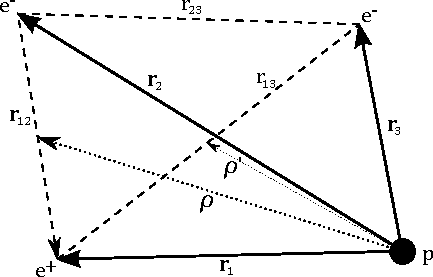
\includegraphics[height=2in]{PsHCoordinates}
	\caption{Positronium-Hydrogen Coordinate System}
	\label{fig:PsHCoords}
\end{figure}

We are investigating low-energy elastic ground-state positronium with ground-state hydrogen (Ps-H) for energies up to the excitation threshold of Ps(n=2) at approximately 5.101 eV. Previous work on Ps-H scattering used the Kohn and inverse Kohn approach \cite{VanReeth2003, VanReeth2004}. The complex Kohn methods are more stable and suffer less from Schwartz singularities than the Kohn, inverse Kohn and generalized Kohn methods \cite{Cooper2010}. All of our final results presented in section \ref{sec:Results} use the S matrix complex Kohn method, but we present a general wavefunction that can be used in any of the variational Kohn methods, as described in section \ref{sec:Kohn}.

For S-wave scattering of positronium from hydrogen, our flexible complex-valued trial scattering wavefunction is
\begin{equation}
\Psi_0^{\pm,t} = \bar{S_0} + L_0^{\pm,t} \, \bar{C}_0 + \sum_{i=1}^{N(\omega)} c_i \phi_{i1},
\label{eq:TrialWave}
\end{equation}
where the superscript $t$ indicates that this is a trial wavefunction. The plus sign indicates the spatially symmetric singlet, and the minus sign indicates the spatially antisymmetric triplet case. The total orbital angular momentum, $L$, is equal to the orbital angular momentum of the incoming Ps, $\ell$. For partial waves $(L = \ell > 0)$,
\begin{equation}
\Psi_\ell^{\pm,t} = \bar{S}_\ell + L^{\pm,t}_\ell \, \bar{C}_\ell + \sum_{i=1}^{N(\omega)} c_{i,\ell} \phi_{i1} + \sum_{i=N(\omega)+1}^{2N(\omega)} d_{i,\ell} \phi_{i2}.
\label{eq:TrialWaveHigher}
\end{equation}
The scattering wavefunctions contain both the long-range terms and short-range correlation terms for small interparticle distances. The coordinate system used in these is shown in figure \ref{fig:PsHCoords}. The variable $\rho$ describes the position of the center of mass of the positronium atom, i.e. $\vec{\rho} = \frac{1}{2}\left(\vec{r_1} + \vec{r_2}\right)$. The long-range terms are given by
\begin{equation}
\label{eq:SCPhiDef}
\begin{bmatrix}
\widetilde{S}_\ell \\ \widetilde{C}_\ell
\end{bmatrix} = u  \begin{bmatrix}
\bar{S}_\ell \\ \bar{C}_\ell
\end{bmatrix} = \begin{bmatrix}
u_{00} & u_{01} \\  u_{10} & u_{11}
\end{bmatrix}
\begin{bmatrix}
\bar{S}_\ell \\ \bar{C}_\ell
\end{bmatrix}, 
\end{equation}
with
\begin{subequations}
\label{eq:SCBarPhiDef}
\begin{align}
\bar{S}_\ell &= \frac{1\pm P_{23}}{\sqrt{2}}Y_{\ell 0}(\theta_\rho,\phi_\rho)\Phi_{Ps,1s}\left(r_{12}\right) \Phi_{H,1S}\left(r_3\right) \sqrt{2\kappa} \,j_\ell\left(\kappa\rho\right) \text{ and} \label{eq:SBar} \\
\bar{C}_\ell &= \frac{1\pm P_{23}}{\sqrt{2}}Y_{\ell 0}(\theta_\rho,\phi_\rho)\Phi_{Ps,1s}\left(r_{12}\right) \Phi_{H,1S}\left(r_3\right) \sqrt{2\kappa} \,n_\ell\left(\kappa\rho\right) f_\ell(\rho). \label{eq:CBar}
\end{align}
\end{subequations}

Note that our generalized T matrix is different than Cooper et al.\ \cite{Cooper2010}, in that our $\bar{S}$ and $\bar{C}$ are swapped, which gives an outgoing wave. \todo{Different location?} $P_{23}$ is the exchange operator for the two electrons. $\Phi_{Ps,1s}\left(r_{12}\right)$ and $\Phi_{H,1s}\left(r_3\right)$ are the ground state wavefunctions of positronium and hydrogen, respectively. The shielding factor, $f_\ell(\rho)$, ensures that the singularity of the Neumann function is removed at the origin and is chosen to be
\begin{equation}
f_\ell(\rho) = \left[1 - \ee^{-\mu \rho} \left(1+\frac{\mu}{2}\rho\right)\right]^{m_\ell}.
\label{eq:PartialWaveShielding}
\end{equation}
The $m_\ell$ is an integer chosen for each $\ell$ so that $\bar{C}$ behaves like $\bar{S}$ as $\rho \rightarrow 0$.

The short-range terms are highly correlated Hylleraas-type functions, including all interparticle distances, given by
\begin{subequations}
\label{eq:PhiDef}
\begin{align}
\bar{\phi}_{ij} &= \left(1 \pm P_{23}\right) Y_{\ell 0}(\theta_j,\phi_j) r_j^{\ell} r_1^{k_i} r_2^{l_i} r_{12}^{m_i} r_3^{n_i} r_{13}^{p_i} r_{23}^{q_i} \label{eq:PartialWavePhi}
\end{align}
\end{subequations}
The variable $\omega$ is an integer $\geq 0$ that determines the maximum number of terms in the basis set. \todo{Needed?} For a chosen value of $\omega$, the integer powers of $r_i$ and $r_{ij}$ are constructed in such a way that $k_i + l_i + m_i + n_i + p_i + q_i \leq \omega$, with all $k_i$, $l_i$, $m_i$, $n_i$, $q_i$ and $p_i$ $\geq 0$. The first symmetry in equation \ref{eq:TrialWaveHigher} has $j = 1$ for $i=1$ to $N(\omega)$, and the second symmetry exists for $\ell > 0$, with $i = N(\omega)$ to $2N(\omega)$.

These short-range terms represent the angular momentum as being placed on either the positron ($r_1$) or on the electron on the Ps atom ($r_2$, and $r_3$ with exchange).
Following up on the NIMB article \cite{VanReeth2004} which had difficulty with convergence for the P-wave triplet, we also tried a wavefunction where the angular momentum was placed on the electron of the H atom ($r_3$) and on the Ps ($\rho$). However, this did not improve convergence for us and was even marginally worse in some cases. The numerical techniques discussed in section \ref{sec:Numerical} improved our convergence.

For partial waves with $L>1$, the angular momentum could be shared between both particles in the Ps atom \cite{Schwartz1961a}. An investigation of the contribution to the final results from each symmetry for e$^+$-Ps scattering \cite{VanReeth1997} has revealed that the mixed symmetries were not important, and because of the complexity of the analytical evaluation of the various matrix elements, we have omitted the mixed symmetry terms where angular momentum is shared.

% THE HAMILTONIAN
The Hamiltonian for the fundamental Coulombic system is
\begin{align}
H = -\frac{1}{2} \nabla_{r_1}^2 - \frac{1}{2} \nabla_{r_2}^2 - \frac{1}{2} \nabla_{r_3}^2 + \frac {1}{r_1}-\frac {1}{r_2}-\frac {1}{r_3}-\frac {1}{r_{12}}-\frac {1}{r_{13}}+\frac {1}{r_{23}}
	\label{Hamiltonian1}
\end{align}
which can also be expressed in terms of the variables associated with the Ps coordinates as
\begin{align}
H = -\frac{1}{4} \nabla_{\rho}^2 - \frac{1}{2} \nabla_{r_3}^2 - \nabla_{r_{12}}^2 + \frac {1}{r_1}-\frac {1}{r_2}-\frac {1}{r_3}-\frac {1}{r_{12}}-\frac {1}{r_{13}}+\frac {1}{r_{23}}
	\label{Hamiltonian2}
\end{align}


\subsection{Kohn Variational Methods}
\label{sec:Kohn}

This derivation follows a similar procedure as that of \cite{Lucchese1989}, \cite{Cooper2010} and \cite{Armour1991}.
The functional for the full wavefunctions in equations \ref{eq:TrialWave} and \ref{eq:TrialWaveHigher} is (dropping the $\ell$ subscript and the $\pm$ superscript for clarity),
\begin{equation}
I[\Psi^t] = \left(\Psi^t, \mathcal{L} \Psi^t \right) = \int \Psi^t \mathcal{L} \Psi^t \,d\tau,
\label{eq:IlDefPsi}
\end{equation}
with
\beq
\mathcal{L} = 2(H - E).
\label{eq:LDef}
\eeq
Notice that the wavefunction is not conjugated, as pointed out by Cooper \emph{et al} \cite{Cooper2010}.

We assume our trial wavefunction is a small variation of the exact wavefunction, or
\beq
\Psi^t = \Psi + \delta \Psi
\label{eq:PsiTrialRelation}
\eeq
It can be shown that solving for $\delta I$, the variation of $I$, gives a result for the variational method of
\beq
\delta I = I[\Psi^t] - I[\Psi] = I[\Psi^t] = (L^t - L + I[\delta \Psi]) \det u.
\label{eq:IlPsiVariation}
\eeq
Neglecting the second order term in $\delta \Psi$ and realizing that $I[\Psi] = 0$, we get a functional for the variational $L^v$ of
\beq
L^v = L^t - I[\Psi^t] / \det u.
\label{eq:ComplexKohnVariation}
\eeq

Using the stationary property of the complex Kohn functional, we get
\beq
\frac{\partial L^v}{\partial L^t} = 0  \text{ and } \frac{\partial L^v}{\partial c_i} = 0 \text{ where $i = 1,\ldots,N$},
\label{eq:ComplexKohnStationary}
\eeq
which can be written as a matrix equation. For the S-wave, this is
\begin{equation}
\label{eq:ComplexKohnMatrix}
\begin{bmatrix} 
 (\widetilde{C},\mathcal{L}\widetilde{C}) & (\widetilde{C},\mathcal{L}\bar{\phi}_1) & \cdots & (\widetilde{C},\mathcal{L}\bar{\phi}_j) & \cdots\\
 (\bar{\phi}_1,\mathcal{L}\widetilde{C}) & (\bar{\phi}_1,\mathcal{L}\bar{\phi}_1) & \cdots & (\bar{\phi}_1,\mathcal{L}\bar{\phi}_j) & \cdots\\
 \vdots & \vdots & \ddots & \vdots \\
 (\bar{\phi}_i,\mathcal{L}\widetilde{C}) & (\bar{\phi}_i,\mathcal{L}\bar{\phi}_1) & \cdots & (\bar{\phi}_i,\mathcal{L}\bar{\phi}_j) & \cdots\\
 \vdots & \vdots & & \vdots & \\
\end{bmatrix}
\begin{bmatrix}
L^t\\
c_1\\
\vdots\\
c_i\\
\vdots
\end{bmatrix}
= -
\begin{bmatrix}
(\widetilde{C},\mathcal{L}\widetilde{S}) \\
(\bar{\phi}_1,\mathcal{L}\widetilde{S}) \\
\vdots \\
(\bar{\phi}_i,\mathcal{L}\widetilde{S}) \\
\vdots
\end{bmatrix}.
\end{equation}
This matrix equation can be rewritten as $\textbf{\emph{AX = -B}}$. For higher partial waves, the matrix equation looks the same but includes the second symmetry short-range terms. Finally, we solve for $L^v$, from which we obtain our phase shifts.
\begin{equation}
L^v = -\frac{1}{\det u} \left( \textbf{\emph{B}}^{tr} \textbf{\emph{X}} + (\widetilde{S},\mathcal{L} \widetilde{S}) \right)
\end{equation}
To determine the phase shifts, we use the relation given by \cite{Lucchese1989} as
\begin{equation}
K_\ell = \tan \delta_\ell = (u_{01} + u_{11} L_\ell)(u_{00} + u_{10} L_\ell)^{-1}.
\end{equation}

%\begin{center}
%\line(1,0){250}
%\end{center}

We use different $u$ matrices to generate multiple Kohn methods, namely the
\begin{align}
&\text{generalized Kohn, } L_\ell = \tan(\delta_\ell-\tau), u = \left[ \begin{smallmatrix}
\cos \tau & \sin \tau \\  -\sin \tau & \cos \tau
\end{smallmatrix} \right], \label{eq:GenKohn}\\
&\text{generalized T matrix Kohn, } L_\ell = T_\ell^\prime, u = \left[ \begin{smallmatrix}
\cos\tau & \sin\tau \\ -\sin\tau + \ii \cos\tau & \cos\tau + \ii \sin\tau
\end{smallmatrix} \right], \label{eq:GenTKohn} \\
\text{and}& \nonumber \\
&\text{generalized S matrix Kohn, } L_\ell = S_\ell^\prime, u = \left[ \begin{smallmatrix}
-\ii \cos\tau - \sin\tau & -\ii\sin\tau + \cos\tau \\ \ii\cos\tau - \sin\tau & \ii\sin\tau + \cos\tau
\end{smallmatrix} \right]. \label{eq:GenSKohn}
\end{align}
For the case of $\tau = 0$, these give the Kohn, the T matrix and the S matrix, respectively. $\tau = \frac{\pi}{2}$ in equation \ref{eq:GenKohn} gives the inverse Kohn.


\subsection{Bound State}
As done earlier by Van Reeth and Humberston \cite{VanReeth2003,VanReeth2004}, we used the short-range correction part of the S-wave scattering wavefunction to compute the binding energy of $^1S$ PsH system. This allows us to determine the reliability of using our short-range terms for the Ps-H scattering problem. The wavefunction we use for the bound state is
\begin{equation}
\label{eq:BoundWavefn}
\Psi^\pm = \sum_{i=1}^{N(\omega)} c_i \phi_{1i}^\pm,
\end{equation}
where $\phi_{1i}^\pm$ is the same as in equation (\ref{eq:PhiDef}). The Rayleigh-Ritz method is used, and the optimization of the nonlinear parameters has been done using the both the Newton and simplex methods \cite{Yan1999,GSL}. For the triplet case and $L \neq 0$, even though there is not a bound state, we use the same method to optimize the nonlinear parameters to get the lowest energy. For $L > 0$, as in the scattering problem, our wavefunction includes both sets of short-range terms for this optimization.


\subsection{Born Approximations}
The Born approximation \cite{?} uses only the first term in equations \ref{eq:TrialWave} and \ref{eq:TrialWaveHigher}. For the Kohn method, this leads to the Born approximation of
\begin{equation}
\label{eq:Born}
\tan\delta_\ell \approx -(\widetilde{S}_\ell,\mathcal{L}\widetilde{S}_\ell )\, .
\end{equation}
We also consider a modified Born approximation that uses the first two terms in equations \ref{eq:TrialWave} and \ref{eq:TrialWaveHigher}, excluding the short-range terms. This gives a better approximation than the Born for most cases and is roughly equivalent to the Born in the other cases.

\subsection{Cross Sections}

We calculate the total elastic cross sections and the elastic differential cross sections using \cite{Bransden2003}, respectively

%\begin{equation}
%\label{eq:PartialCross}
%\sigma_\ell^\pm = \frac{4(2\ell+1)}{\kappa^2} \sin^2 \delta_\ell^\pm
%\end{equation}

\begin{equation}
\label{eq:TotalCross}
\sigma^\pm = \frac{4}{\kappa^2} \sum_{\ell=0}^\infty (2\ell+1) \sin^2 \delta_\ell^\pm
\end{equation}
and
\begin{align}
\label{eq:DiffCross}
\nonumber \frac{d\sigma^\pm}{d\Omega} = \frac{1}{\kappa^2} & \sum_{\ell=0}^\infty \sum_{\ell^\prime=0}^\infty (2\ell+1)(2\ell^\prime+1) \exp\left\{\ii \left[\delta_\ell(\kappa) - \delta_{\ell^\prime}(\kappa) \right] \right\} \\
& \times \sin\delta_\ell^\pm(\kappa) \sin\delta_{\ell^\prime}^\pm(\kappa) P_\ell(\cos\theta) P_{\ell^\prime}(\cos\theta)\,.
\end{align}
Equation \ref{eq:TotalCross} is in units of $\pi a_0^2$, and equation \ref{eq:DiffCross} is in units of $\pi a_0^2 / \rm{sr}$. The singlet for each of the partial waves contributes $1/4$ to the total and differential cross sections, while the triplet contributes $3/4$.


\subsection{Effective Range}


\section{Numerics}
\label{sec:Numerical}
%Describe Todd's procedure.
%How terms are eliminated for the bound-state
%and give the procedure for determining the
%number for the scattering.
%Give a table for the number of terms for bound-state,
%for singlet and triplet scattering.
%Compare with the total number of terms,
%and the number of terms that Peter considered.
%Explain how the non-linear terms are obtained for the
%bound-state, singlet and triplet scattering.
%\todoi{Compare with the nonlinear parameters that Peter used.}
%\vskip 1truecm
%\noindent

\subsection{Short-Short Integrations}
\label{sec:ShortInt}
For the PsH bound state and S-wave, we use the efficient asymptotic expansion method presented by Drake and Yan \cite{Drake1995} for the evaluation of correlated integrals of the form
\begin{equation}
\label{eq:ShortInt}
I(j_1,j_2,j_3,j_{12},j_{23},j_{31}; \bar{\alpha}, \bar{\beta}, \bar{\gamma}) =
\int
d \textbf{r}_1 d \textbf{r}_2 d \textbf{r}_3
r_1^{j_1} r_2^{j_2} r_3^{j_3} r_{12}^{j_{12}}
r_{23}^{j_{23}} r_{31}^{j_{31}}
e^{-(\bar{\alpha} r_1 + \bar{\beta} r_2 + \bar{\gamma} r_3)}\, .
\end{equation}
These integrals arise from evaluation of the matrix elements $(\phi_i, L \phi_j)$, $(\phi_i, H \phi_j)$ and $(\phi_i, \phi_j)$, where $H$ is the full Hamiltonian of the system,
which is needed in both the bound state and scattering calculations. To verify our calculation of these integrals, we have also used the recursion relations of Pachucki \cite{Pachucki2004}.

For $L > 0$, we use two different methods to perform these integrations. The first is to perform rotations and then integrate over external angles, reducing these integrals down to the form of equation \ref{eq:ShortInt}. We then use the asymptotic expansion method to solve. This works through the D-wave. For higher L, we use a second method from Yan and Drake \cite{Yan1997}. These integrals have the form of
\begin{align}
\label{eq:ShortIntGen}
\nonumber I(\ell_1^\prime m_1^\prime, & \ell_2^\prime m_2^\prime, \ell_3^\prime m_3^\prime; j_1,j_2,j_3,j_{12},j_{23},j_{31}; \bar{\alpha}, \bar{\beta}, \bar{\gamma}) \\
\nonumber = & \int
d \textit{\textbf{r}}_1 d \textit{\textbf{r}}_2 d \textit{\textbf{r}}_3
r_1^{j_1} r_2^{j_2} r_3^{j_3} r_{12}^{j_{12}}
r_{23}^{j_{23}} r_{31}^{j_{31}}
e^{-(\bar{\alpha} r_1 + \bar{\beta} r_2 + \bar{\gamma} r_3)} \\
& \times Y_{\ell_1^\prime m_1^\prime}^* (\textit{\textbf{r}}_1) Y_{\ell_2^\prime m_2^\prime}^* (\textit{\textbf{r}}_2) Y_{\ell_3^\prime m_3^\prime}^* (\textit{\textbf{r}}_3)
Y_{\ell_1 m_1} (\textit{\textbf{r}}_1) Y_{\ell_2 m_2} (\textit{\textbf{r}}_2) Y_{\ell_3 m_3} (\textit{\textbf{r}}_3)\, .
\end{align}

\subsection{Long-Range Integrations}
\label{sec:LongInt}
The long-range--long-range and short-range--long-range matrix elements in equations \ref{eq:ComplexKohnMatrix} and \ref{eq:GenKohnMatrix} are evaluted using Gauss-Laguerre and Gauss-Legendre quadratures. Due to a cusp in the integrands, the $r_2$ and $r_3$ integrations are split into Gauss-Legendre quadratures before the cusp and Gauss-Laguerre after the cusp. \todo{Always true?} Previous calculations \cite{VanReeth2003,VanReeth2004} treated these cusps as unimportant at 25 au, while we have extended it to 100 au before we consider them important.

To further improve the convergence of the short-range--long-range matrix elements, we investigated the integrands. The biggest source of difficulty in converging these results comes through the Gaussian-Laguerre quadratures in the $r_1$, $r_2$ and $r_3$ integrations. Specifically, the integrands do not fall off quickly enough, and the tails of the integrands are not adequately represented. This can be resolved by introducing more abscissae in the quadratures, which puts some points farther out. This brute force approach can increase the computational time greatly, so we took another approach to further increase the accuracy. For each of the Gauss-Laguerre quadratures, we introduce an extra $e^{-\lambda r_i}$ and remove it with $e^{\lambda r_i}$ after the quadrature, pushing our abscissae further out without increasing the number of integration points.



\subsection{Todd's procedure}
\label{sec:Todd}
We use a method from Todd \cite{Todd2007} to remove short-range terms that contribute to linear dependence. This is a variation of the procedure from L\"uchow and Kleindienst \cite{Luchow1992}. They use multiple blocks, while we optimize with a single block. They also use a criteria of $\Delta E$ to determine when to discard terms. Instead, we compare the lowest eigenvalues from the separate calculations using the upper and lower triangular matrices in LAPACK's \texttt{dsygv} routine \cite{LAPACK}, discarding terms when they cause the difference to be greater than a predetermined threshold. The reordering introduced by this method is referred to as ``Todd ordering'' in this paper, as compared to the original ordering indicated by increasing $\omega$.


\subsection{Selection of Short-Range Terms}
\label{sec:Truncation}
We have observed that the short-range--short-range terms used in the same order as the output of the Todd algorithm will generate better-converged phase shifts, and we can include more short-range terms before linear dependence becomes a problem. The phase shifts are calculated using this set of short-range terms for the generalized Kohn variational method for multiple $\tau$ values. We further truncate this basis set where the phase shifts for the different Kohn methods begin to diverge. This can be seen in figure \ref{??}. The final results in section \ref{sec:Results} use the S matrix complex Kohn with this set of short-range terms.

\todoi{Graphs of with and without Todd ordering for energy and phase shifts?}

For the S-wave singlet, we noticed an additional property of the phase shift graphs. When $\delta_0^+$ is plotted for one Kohn method with respect to $N(\omega)$ for multiple $\mu$ values, the phase shifts agree well for the different $\mu$ values up until linear dependence becomes apparent. We used this criteria to determine where to truncate the basis set, stopping at 1505 terms for $^1S$. We did not see a similar effect for the S-wave triplet.


\subsection{Fittings}
As with the previous Kohn calculation of Van Reeth and Humberston \cite{VanReeth2004}, we fitted our computed phase shifts for the S-wave and P-wave to the resonance formula
\begin{equation}
\label{eq:ResonanceFit}
\delta(E) = A + B E + C E^2 + \arctan \left[ \frac{^1\Gamma}{2(^1E_R - E)} \right] + \arctan \left[ \frac{^2\Gamma}{2(^2E_R - E)} \right]
\end{equation}
to extract out the positions ($^1E_R$ and $^2E_R$) and widths
($^1\Gamma$ and $^2\Gamma$) of the two resonances. 
This formula is comprised of the Breit-Wigner resonance
formula for the two resonances and allows for a slowly varying
background. The D-wave and F-wave resonance fits were performed without the second $\arctan$ term, as they have a single resonance. 
The data from each variant of the Kohn variational methods was fitted using the MATLAB nonlinear fitting routine \texttt{nlinfit} with eight possible weightings.
For each variant of the Kohn variational method, the four parameters were determined for each of the eight fits and compared.

For each variant of the Kohn method, we extrapolated the phase shifts in tables \ref{tab:SWavePhase} and \ref{} according to the empirical formula \cite{VanReeth2003}
\begin{equation}
\label{eq:Extrap}
\tan\delta_\ell^\pm(\omega) = \tan\delta_\ell^\pm(\omega\to\infty) + {c\over \omega^p}\, .
\end{equation}


\subsection{Nonlinear Parameters and Terms Used}
\label{sec:Parameters}

\begin{table}[H]
  \centering
	\begin{ruledtabular}
    \begin{tabular}{cccccccccc}
    Parameter & $^1S$ & $^3S$ & $^1P$ & $^3P$ & $^1D$ & $^3D$ & $^1F$, $^3F$ & $^1G$, $^3G$ & $^1H$, $^3H$ \\
    \colrule
	$\omega$           & 7     & 7     & 7     & 7     & 6     & 6     & 5    & 5   & 5 \\
	$N^\prime(\omega)$ & 1505  & 1633  & 1000  & 1000  & 916   & 919   & 462  & 462 & 462 \\
	$\alpha$           & 0.586 & 0.323 & 0.397 & 0.310 & 0.359 & 0.356 & 0.5  & 0.5 & 0.5 \\
	$\beta$            & 0.580 & 0.334 & 0.376 & 0.311 & 0.368 & 0.365 & 0.6  & 0.6 & 0.6 \\
	$\gamma$           & 1.093 & 0.975 & 0.962 & 0.995 & 0.976 & 0.976 & 1.1  & 1.1 & 1.1 \\
	$\mu$              & 0.9   & 0.9   & 0.9   & 0.9   & 0.7   & 0.7   & 0.7  & 0.7 & 0.7 \\
	$m_\ell$           & 1     & 1     & 3     & 3     & 7     & 7     & 7    & 9   & 11 \\
    \end{tabular}
  \end{ruledtabular}
  \caption{Parameters for each partial wave}
  \label{tab:Nonlinear}
\end{table}





\section{Results}
\label{sec:Results}


\subsection{Bound State Results}

The Rayleigh-Ritz variational method provides a true bound on the total energy and binding energy. The total energy and binding energy converges well with respect to $\omega$. To be consistent with the scattering calculation, we report the results obtained with the same set of nonlinear parameters that were used in the scattering calculation, namely $\alpha = 0.586$, $\beta = 0.580$ and $\gamma = 1.093$. We note that we are able to obtain a slightly better value for the binding energy with higher $\omega$, but we are unable to use this many terms in the full scattering calculations for Ps-H. Table \ref{tab:BoundEnergy} compares our energies for PsH with that obtained by other groups.

Our calculation yields a better value for these
quantities than the earlier variational calculation \cite{VanReeth2003,VanReeth2004}
but not as good as the variational calculation of
Yan and Ho, who also used Hylleraas wave functions \cite{Yan1999}.
While we do not obtain the best value of the binding energy
(this was not the purpose of our calculation),
we obtained results for this quantity which compare favorably with
the most elaborate calculation in the literature which
used 5000 explicitly correlated Gaussians \cite{Bubin2006}.
Our calculation of the binding energy gave us confidence
in the reliability of the short-range part of the
scattering wave function to describe
the $^1S$ PsH system.


\squeezetable  % Makes the table smaller
\begin{table}[H]
\begin{center}
%\begin{tabular}{|l|l|c|l|l|}
\begin{ruledtabular}  % From http://www.latex-community.org/forum/viewtopic.php?f=45&t=20722
\begin{tabular}{l l c l l}
%\toprule
Group & Method & Terms & Total Energy (au) & Binding Energy (eV)\\
%\hline
\colrule
%\midrule
Ho (1986) \cite{Ho1986} & Variational with Hylleraas (?) & 396 & -0.788 945$^\star$ & 1.059 75 \\
Yan (1999) \cite{Yan1999} & Variational with Hylleraas $(\omega \rightarrow \infty)$ & --- & -0.789 196 714 7$^\star$ & 1.066 596 896 \\
Blackwood (2002) \cite{Blackwood2002} & Close-coupling 14Ps14H & --- & -0.786 5 & 0.994$^\star$ \\
Van Reeth (2003) \cite{VanReeth2003} & Variational with Hylleraas $(\omega = 6)$ & 721 & -0.789 156 & 1.0655$^\star$ \\
Walters (2004) \cite{Walters2004} & Close-coupling 14Ps14H + $\text{H}^-$ & --- & -0.787 9 & 1.03$^\star$\\
Mitroy (2006) \cite{Mitroy2006} & ECGs with SVM & 1800 & -0.789 196 740$^\star$ & 1.066 597 58 \\
Bubin (2006) \cite{Bubin2006} & ECGs variational & 5000 & -0.789 196 765 251$^\star$ & 1.066 598 271 959 \\
Current work & Variational with Hylleraas & 1505 & -0.789 189 725 & 1.066 406 705 \\
%\bottomrule
\end{tabular}
\end{ruledtabular}
\caption{Positronium hydride energy comparisons. Starred values are the reported values, and unstarred values are obtained by using the conversion factor given in \cite{NISTConversions}.}
\label{tab:BoundEnergy}
\end{center}
\end{table}

\todoi{Do we need to include terms?}


\subsection{Phase Shifts}

In table \ref{tab:SWavePhase}, we show the singlet and triplet S-wave phase shifts using the S matrix Kohn variational method. To the accuracy given, the results agree from the various methods described in section \ref{sec:Kohn}, after removing any obvious Schwartz singularities. The extrapolated values to estimate the phase shifts at $\omega = \infty$ were obtained for $\omega = 4$ to $\omega = 7$ using equation \ref{eq:Extrap}. By computing the percentage difference between the extrapolated phase shifts and the computed phase shifts at $\omega=7$, we estimate that the $^1S$ phase shifts have converged to better than about $0.22\%$ for the range $\kappa=0.1$ to $0.7$ and that the $^3S$ phase shifts have converged to better than $0.27\%$ for the same range of $\kappa$.

In this table, we also compare our results with the earlier Kohn variational results \cite{VanReeth2003,VanReeth2004} and with the elaborate close-coupling results of Walters' group \cite{Blackwood2002,Walters2004}. Our new $\omega = 7$ results are in excellent agreement with the earlier Kohn $\omega = 6$ variational results, being either identical or slightly lower, indicating that the earlier S-wave calculations were well-converged.


The slight difference in phase shifts between the previous and current Kohn methods can be attributed to two factors. Using Todd's procedure (described in section \ref{sec:Todd}) allowed us to use more terms (see table \ref{tab:Nonlinear}) than the earlier Kohn calculations, which used 721 terms \todo{in paper?} \cite{VanReeth2003}. This slightly increased the phase shifts, but we also used more integration points in these calculations, slightly decreasing the phase shifts.

The Kohn results are in good agreement with the close-coupling results of the Walters group \cite{Blackwood2002,Walters2004}. For the singlet, the Kohn phase shifts are slightly larger than the close-coupling results. Because of the empirical bounds on the
Kohn variational results and, in practice on
the close-coupling (except for the Buttle
correction), the Kohn results could be
slightly more accurate than the close-coupling.
The situation is reversed for the triplet.
In this case, the Kohn results are slightly
more negative than the close-coupling results.
However, the Kohn and close-coupling results are
in very good agreement.

The recent confined variational S-wave results from Zhang and Yan \cite{Zhang2012} agree extremely well with the Kohn results, even for the triplet, potentially indicating that the Kohn results are more accurate than the close-coupling. Figure \ref{fig:swave-phases} shows the full range of our calculations, with comparisons to the close-coupling and confined variational results. Excellent agreement between the three sets of results is evident.
\todoi{More about this? Shouldn't the confined variational be in the table?} 

The figure shows two $^1S$ Rydberg \todo{?} resonances below the
Ps(n=2) + H(n=1) channel
and associated
with the ... \todo{which?} threshold.
(These resonances results were also obtained in the CC calculations,
which obtain three resonances. check.)
These resonances were first computed by
Drachman and Houston using the stabilization
method and complex rotation method.
They have recently been computed very accurately
by Yan and Ho
using the complex rotation method who
obtain the first three of the infinite
number of Rydberg resonances (as did the CC (check)).
\todoi{This paragraph needs to be rewritten and maybe moved to the resonances section.}

In figures \ref{fig:OtherSWaveSingletResults} and \ref{fig:OtherSWaveTripletResults}, respectively,
we compare the singlet and triplet S-wave phase shifts obtained from the Kohn variational
method (and variants) with various other calculations. \todoi{Compare?}

Tables \ref{tab:PWavePhase} and \ref{tab:DWavePhase} show our phase shifts for the P-wave and D-wave, respectively. The small percentage differences with the extrapolated values indicates that our phase shifts are well converged. Similar to the S-wave, the $^1$P phase shifts are slightly above the close-coupling results, and our $^3$P phase shifts are below. Figure \ref{fig:pwave-phases} shows that the Kohn and CC results agree well. We are unable to perform an extrapolation on the D-wave phase shifts, but we expect that they are reasonably well converged. Both the $^1$D and $^3$D phase shifts are below the CC. Figure \ref{fig:dwave-phases} shows that the Kohn and CC also agree reasonably well. \todoi{What else should we say about this?}


\begin{table}[H]
\centering
\begin{ruledtabular}
\begin{tabular}{c c c c c c c}
$\kappa$ (au) & $\delta_0^+ (\omega = 7)$ & $\delta_0^+ (\omega =\infty)$ & \% Diff$^+$ & $\delta_0^+$ (VH) & $\delta_0^+$ (WYSG) & $\delta_0^+$ (Zhang)\\
\colrule
0.1 & -0.427 & -0.426 & 0.223\% & -0.427 & -0.432 & -0.42636 \\
0.2 & -0.820 & -0.819 & 0.010\% & -0.820 & -0.833 & -0.81973 \\
0.3 & -1.161 & -1.161 & 0.040\% & -1.161 & -1.179 & \\
0.4 & -1.446 & -1.446 & 0.022\% & -1.446 & -1.466 & \\
0.5 & -1.678 & -1.677 & 0.031\% & -1.677 & -1.699 & \\
0.6 & -1.858 & -1.857 & 0.040\% & -1.857 & -1.884 & \\
0.7 & -1.964 & -1.963 & 0.045\% & -1.964 & -2.012 & \\
\end{tabular}
\end{ruledtabular}
\caption{S-wave singlet phase shifts}
\label{tab:SWaveSingletPhase}
\end{table}


\begin{table}[H]
\centering
\begin{ruledtabular}
\begin{tabular}{c c c c c c c}
$\kappa$ (au) & $\delta_0^- (\omega = 7)$ & $\delta_0^- (\omega = \infty)$ & \% Diff$^-$ & $\delta_0^-$ (VH) & $\delta_0^-$ (BMW) & $\delta_0^-$ (Zhang) \\
\colrule
0.1 & -0.215 & -0.214 & 0.120\% & -0.214 & -0.206 & -0.21464 \\
0.2 & -0.431 & -0.431 & 0.063\% & -0.432 & -0.414 & -0.43159 \\
0.3 & -0.645 & -0.645 & 0.094\% & -0.645 & -0.624 & \\
0.4 & -0.850 & -0.849 & 0.130\% & -0.850 & -0.838 & \\
0.5 & -1.041 & -1.040 & 0.166\% & -1.040 & -1.037 & \\
0.6 & -1.217 & -1.214 & 0.273\% & -1.215 & -1.213 & \\
0.7 & -1.375 & -1.372 & 0.250\% & -1.373 & -1.367 & \\
\end{tabular}
\end{ruledtabular}
\caption{S-wave triplet phase shifts}
\label{tab:SWaveTripletPhase}
\end{table}


\begin{table}[H]
\begin{center}
\begin{ruledtabular}
\begin{tabular}{c c c c c c c c c c}
$\kappa$ (au) & $\delta_1^+ (\omega = 7)$ & $\delta_1^+ (\omega = \infty)$ & \% Diff$^+$ & $\delta_1^+$ (WYSG) & $\delta_1^- (\omega = 7)$ & $\delta_1^- (\omega = \infty)$ & \% Diff$^-$ & $\delta_1^-$ (BMW) \\
\colrule
0.1 & $0.226^{-1}$ & $0.227^{-1}$ & $0.465\%$ & $0.221^{-1}$ & $-0.178^{-2}$ & $-0.172^{-2}$ & $3.176\%$ & $-0.953^{-3}$ \\
0.2 & $0.191$      & $0.192$      & $0.306\%$ & $0.183$      & $-0.167^{-1}$ & $-0.165^{-1}$ & $0.993\%$ & $-0.122^{-1}$ \\
0.3 & $0.609$      & $0.611$      & $0.314\%$ & $0.580$      & $-0.552^{-1}$ & $-0.540^{-1}$ & $0.749\%$ & $-0.456^{-1}$ \\
0.4 & $0.994$      & $0.996$      & $0.205\%$ & $0.956$      & $-0.115$      & $-0.114$      & $0.698\%$ & $-0.104$ \\
0.5 & $1.140$      & $1.142$      & $0.140\%$ & $1.106$      & $-0.183$      & $-0.182$      & $0.749\%$ & $-0.178$ \\
0.6 & $1.162$      & $1.163$      & $0.137\%$ & $1.134$      & $-0.248$      & $-0.246$      & $0.896\%$ & $-0.247$ \\
0.7 & $1.152$      & $1.154$      & $0.181\%$ & $1.133$      & $-0.292$      & $-0.281$      & $1.237\%$ & $-0.295$ \\
\end{tabular}
\end{ruledtabular}
\caption{P-wave singlet and triplet phase shifts}
\label{tab:PWavePhase}
\end{center}
\end{table}


\begin{table}[H]
\begin{center}
\begin{ruledtabular}
\begin{tabular}{c c c c c}
$\kappa$ (au) & $\delta_2^+ (\omega = 6)$ & $\delta_2^+$ (WYSG) & $\delta_2^- (\omega = 6)$ & $\delta_2^-$ (BMW) \\
\colrule
$0.1$ & $1.358^{-4}$ & $1.46^{-4}$ & $5.808^{-5}$ & $8.48^{-5}$ \\
$0.2$ & $2.987^{-3}$ & $3.15^{-3}$ & $7.120^{-4}$ & $1.15^{-3}$ \\
$0.3$ & $1.592^{-2}$ & $1.65^{-2}$ & $1.065^{-3}$ & $2.84^{-3}$ \\
$0.4$ & $4.933^{-2}$ & $4.95^{-2}$ & $-2.002^{-3}$ & $2.37^{-3}$ \\
$0.5$ & $1.113^{-1}$ & $1.08^{-1}$ & $-1.122^{-2}$ & $-4.66^{-3}$ \\
$0.6$ & $2.027^{-1}$ & $1.94^{-1}$ & $-2.647^{-2}$ & $-1.85^{-2}$ \\
$0.7$ & $3.215^{-1}$ & $3.02^{-1}$ & $-4.451^{-2}$ & $-3.27^{-2}$ \\
\end{tabular}
\end{ruledtabular}
\caption{D-wave singlet and triplet phase shifts}
\label{tab:DWavePhase}
\end{center}
\end{table}


\begin{figure}[ht]
	\centering
	\includegraphics[width=3.4in]{swave-phases}
	\caption{S-wave singlet and triplet phase shifts}
	\label{fig:swave-phases}
\end{figure}

\begin{figure}[H]
	\centering
	\includegraphics[width=3.4in]{OtherSWaveSingletResults}
	\caption{Comparison of S-wave singlet results from other groups}
	\label{fig:OtherSWaveSingletResults}
\end{figure}

\begin{figure}[H]
	\centering
	\includegraphics[width=3.4in]{OtherSWaveTripletResults}
	\caption{Comparison of S-wave triplet results from other groups}
	\label{fig:OtherSWaveTripletResults}
\end{figure}
\todoi{Need this one?}


\begin{figure}[H]
	\centering
	\includegraphics[width=3.4in]{pwave-phases}
	\caption{P-wave singlet and triplet phase shifts}
	\label{fig:pwave-phases}
\end{figure}


\begin{figure}[H]
	\centering
	\includegraphics[width=3.4in]{dwave-phases}
	\caption{D-wave singlet and triplet phase shifts}
	\label{fig:dwave-phases}
\end{figure}

Figures \ref{fig:fwave-phases}, \ref{fig:gwave-phases}, and \ref{fig:hwave-phases} show the F-wave, G-wave and H-wave phase shifts compared to the Born approximation. Even for these higher partial waves, the Born approximation is not particularly good, being much lower. The Born approximation does not even have the correct sign for the phase shifts for the G-wave and H-wave triplet. This comparison is not shown for the first three partial waves, as there is very little agreement. The F-wave has a resonance above the Ps(n=2) threshold, but the beginning of the resonance is evident in figure \ref{fig:fwave-phases}.

We performed full Kohn calculations on all first six partial waves, but we did more extensive calculations for the first three partial waves, as shown by the parameters and terms used in section \ref{sec:Parameters}. For the F-wave through the H-wave, the phase shifts and partial elastic cross sections become very small, so their overall contribution to the total elastic cross sections becomes mostly negligible by the G-wave. The G-wave only contributes up to 0.001\% to the total elastic cross sections at the most.
\todoi{Check the percentage}

The differential cross sections shown in figures \ref{fig:diff-cross-section-2D-theta}, \ref{fig:diff-cross-section-2D-kappa}, and \ref{fig:combined-diff-cross-sections} require more partial waves, and the contributions to these do not become negligible until the H-wave. 

\begin{figure}[H]
	\centering
	\includegraphics[width=3.4in]{fwave-phases}
	\caption{F-wave singlet and triplet phase shifts}
	\label{fig:fwave-phases}
\end{figure}

\todoi{Mention how e$^+$-H and e$^+$-He First Born (electron too?) higher partial waves similar to Kohn - moreso than ours}

\begin{figure}[H]
	\centering
	\includegraphics[width=3.4in]{gwave-phases}
	\caption{G-wave singlet and triplet phase shifts}
	\label{fig:gwave-phases}
\end{figure}

\begin{figure}[H]
	\centering
	\includegraphics[width=3.4in]{hwave-phases}
	\caption{H-wave singlet and triplet phase shifts}
	\label{fig:hwave-phases}
\end{figure}


\begin{figure}[H]
	\centering
	\includegraphics[width=3.4in]{combined-cross-sections}
	\caption{Total elastic cross sections}
	\label{fig:combined-cross-sections}
\end{figure}

The Walters data \cite{Walters2004} in figure \ref{fig:combined-cross-sections} was extracted from their paper using the CurveSnap program \cite{CurveSnap}.
\todoi{Maximum percentages each higher partial wave contributed to the cross sections and differential cross sections}

\begin{figure}[H]
	\centering
	\includegraphics[width=3.4in]{diff-cross-section-2D-theta}
	\caption{Elastic differential cross sections for selected angles}
	\label{fig:diff-cross-section-2D-theta}
\end{figure}

\begin{figure}[H]
	\centering
	\includegraphics[width=3.4in]{diff-cross-section-2D-kappa}
	\caption{Elastic differential cross sections for selected incident Ps momenta}
	\label{fig:diff-cross-section-2D-kappa}
\end{figure}

\begin{figure}[H]
	\centering
	\includegraphics[width=3.4in]{combined-diff-cross-sections}
	\caption{Elastic differential cross sections}
	\label{fig:combined-diff-cross-sections}
\end{figure}

\begin{figure}[H]
	\centering
	\includegraphics[width=3.4in]{orthopara-cross-sections}
	\caption{Ortho-Para Conversion Cross Sections}
	\label{fig:orthopara-cross-sections}
\end{figure}

\begin{figure}[H]
	\centering
	\includegraphics[width=3.4in]{momentum-cross-sections}
	\caption{Momentum transfer cross sections}
	\label{fig:momentum-cross-sections}
\end{figure}








%In figure \ref{}, we compare the Kohn variational
%$^1S$ S-wave phase shifts computed with $\omega = 7$
%with the close-coupling results.
%Excellent agreement between the
%two sets of results is evident.
%The figure show two $^1S$ Rydberg resonance below the
%Ps(n=2) + H(n=1) channel
%and associated
%with the ... \todo{which?} threshold.
%(These resonances results were also obtained in the CC calculations,
%which obtain three resonances. check.)
%These resonances were first computed by
%Drachman and Houston using the stabilization
%method and complex rotation method.
%They have recently been computed very accurately
%by Yan and Ho
%using the complex rotation method who
%obtain the first three of the infinite
%number of Rydberg resonances (as did the CC (check)).


\subsection{Resonances}

\todoi{Mention source of resonances from Di Rienzi / Drachman \cite{DiRienzi2002b}}

The singlet S-wave and P-wave have two resonances each before the Ps(n=2) threshold, and the D-wave has one resonance before. The F-wave has a resonance just after the threshold. We fit the phase shifts in the resonance region to equation \ref{eq:ResonanceFit} for the S-wave and P-wave. The D-wave and F-wave resonance fits were performed without the second arctan term, as they have a single resonance.

In tables \ref{tab:SWaveResonances}, \ref{tab:PWaveResonances}, \ref{tab:DWaveResonances}, and \ref{tab:FWaveResonances}, we give our calculations of the resonance parameters and compare with other calculations. The values we give for the parameters are the average values from the variants of the Kohn variational method described in section \ref{sec:Kohn}. Data that has Schwartz singularities is removed before fitting. For the errors quoted in these tables, we give the standard deviation obtained from the data sets.

Excellent agreement is achieved between the parameters obtained with between the two sets of Kohn calculations (present and earlier). Good agreement is achieved between the resonance positions obtained with the complex rotation calculations of Yan and Ho \cite{Yan1999,Yan1998a,Ho1998,Ho2000} and our work. There is less agreement with the resonance width for the second resonance in the P-wave calculation, which is a narrow resonance.

The close-coupling results, 9HPsPs \cite{Blackwood2002} and 9H9Ps+H$^-$ \cite{Walters2004}, are comparable to the Kohn and complex rotation calculations. This comparison confirms the importance of the H$^-$ channel in bringing the position of the first resonance, $^1E_R$, into better agreement with the Kohn and complex rotation calculations.

We observed no resonances in the triplet for any of these partial waves, which is consistent with the discussion by Blackwood et al. \cite{Blackwood2002}, who predicted that there should be no resonances for the triplet. Ray \cite{Ray2006} obtained a triplet resonance in a 3-state close-coupling approximation, but we see no evidence of this resonance.

\begin{table}[H]
\begin{center}
\begin{ruledtabular}
\begin{tabular}{l c c c c c}
Method & $^1E_R \text{ (eV)}$ & $^1\Gamma \text{ (eV)}$ & $^2E_R \text{ (eV)}$ & $^2\Gamma \text{ (eV)}$ \\
\colrule
Current work & $4.0065 \pm 0.0001$ & $0.0955 \pm 0.0001$ & $5.0277 \pm 0.0018$ & $0.0608 \pm 0.0005$ \\
Complex rotation (Yan and Ho 1999) \cite{Yan1999} $^\dagger$ & $4.0058 \pm 0.0005$ & $0.0952 \pm 0.0011$ & $4.9479 \pm 0.0014$ & $0.0585 \pm 0.0027$ \\
Stabilization (Yan and Ho 2003) \cite{Yan2003} & $4.007$ & $0.0969$ & $4.953$ & $0.0574$ \\
Kohn variational (Van Reeth and Humberston 2004) \cite{VanReeth2004} & $4.0072 \pm 0.0020$ & $0.0956 \pm 0.010$ & $5.0267 \pm 0.0020$ & $0.0597 \pm 0.0010$ \\
Close coupling (Walters \emph{et al} 2004) \cite{Walters2004} & $4.149$ & $0.103$ & $4.877$ & $0.0164$ \\
\end{tabular}
\end{ruledtabular}
\caption{S-Wave Resonance Parameters} % title of Table
\label{tab:SWaveResonances}
\end{center}
\end{table}


\begin{table}[H]
\begin{center}
\begin{ruledtabular}
\begin{tabular}{l c c c c c}
Method & $^1E_R \text{ (eV)}$ & $^1\Gamma \text{ (eV)}$ & $^2E_R \text{ (eV)}$ & $^2\Gamma \text{ (eV)}$ \\
\colrule
Current work & $4.2856 \pm 0.0001$ & $0.0444 \pm 0.0001$ & $5.0578 \pm 0.0001$ & $0.0456 \pm 0.0002$ \\
Complex rotation (Yan \emph{et al} 1998) \cite{Yan1999} $^\dagger$ & $4.2850 \pm 0.0014$ & $0.0435 \pm 0.0027$ & $5.0540 \pm 0.0027$ & $0.0925 \pm 0.0054$ \\
Stabilization (Yan and Ho 2003) \cite{Yan2003} & $4.287$ & $0.0446$ & $5.062$ & $0.0563$ \\
Close coupling (Walters \emph{et al} 2004 \cite{Walters2004}) & $4.475$ & $0.0827$ & $4.905$ & $0.0043$ \\
Kohn (Van Reeth \emph{et al} 2004) \cite{VanReeth2004} & $4.29 \pm 0.01$ & $0.042 \pm 0.005$ & --- & --- \\
\end{tabular}
\end{ruledtabular}
\caption{P-Wave Resonance Parameters} % title of Table
\label{tab:PWaveResonances}
\end{center}
\end{table}


\begin{table}[H]
\begin{center}
\begin{ruledtabular}
\begin{tabular}{l c c}
Method & $^1E_R \text{ (eV)}$ & $^1\Gamma \text{ (eV)}$ \\
\colrule
Current work & $4.7189 \pm 0.0002$ & $0.0860 \pm 0.0005$ \\
Complex rotation (Yan \emph{et al} 1998) \cite{Ho1998} & $4.710 \pm 0.0027$ & $0.0925 \pm 0.0054$  \\
Stabilization (Yan and Ho 2003) \cite{Yan2003} & $4.714$ & $0.0969$ \\
Close coupling (Walters \emph{et al} 2004 \cite{Walters2004}) & $4.899$ & $0.0872$ \\
\end{tabular}
\end{ruledtabular}
\caption{D-Wave Resonance Parameters} % title of Table
\label{tab:DWaveResonances}
\end{center}
\end{table}


\begin{table}[H]
\begin{center}
\begin{ruledtabular}
\begin{tabular}{l c c}
Method & $^1E_R \text{ (eV)}$ & $^1\Gamma \text{ (eV)}$ \\
\colrule
Current work $(\omega = 6)$ & $5.1822$ & $0.0107$ \\
Complex rotation (Ho and Yan 2000) \cite{Ho2000} & $5.1661 \pm 0.0014$ & $0.0174 \pm 0.0027$  \\
Close coupling (Walters \emph{et al} 2004 \cite{Walters2004}) & $5.200$ & $0.0095$ \\
\end{tabular}
\end{ruledtabular}
\caption{F-Wave Resonance Parameters} % title of Table
\label{tab:FWaveResonances}
\end{center}
\end{table}



\todoi{Do we want to do partial wave cross sections, like \cite{Blackwood2002}?}


\section{Effective Range Theory}

\begin{table}[H]
\begin{center}
\begin{ruledtabular}
\begin{tabular}{c c c c c c}
Partial Wave & $\omega$ & $a^+ (\kappa = 0.001)$ & $a^+ (\kappa = 0.0001)$ & $a^- (\kappa = 0.001)$ & $a^- (\kappa = 0.0001)$ \\
\colrule
S & 7 & 4.3306 & 4.3306 & 2.1363 & 2.1363 \\
P & 7 & -22.089 & --- & 1.4885 & --- \\
\end{tabular}
\end{ruledtabular}
\caption{Scattering Lengths from $-\tan \delta^\pm\kappa$}
\label{tab:ScatLenDef}
\end{center}
\end{table}

\begin{table}[H]
\begin{center}
\begin{ruledtabular}
\begin{tabular}{l l l l l}
Method & \multicolumn{1}{c}{$a^+$} & \multicolumn{1}{c}{$r_0^+$} & \multicolumn{1}{c}{$a^-$} & \multicolumn{1}{c}{$r_0^-$}\\
\colrule
Static-exchange (Hara \emph{et al} 1975) \cite{Hara1975} & 7.275 & \,\,--- & 2.476 & \,\,--- \\
Kohn 35 terms (Page 1976) \cite{Page1976} & 5.844 & 2.90 & 2.319 & \,\,--- \\
Stabilization (Drachman \emph{et al} 1975) \cite{Drachman1975} & 5.33 & 2.54 & \,\,--- & \,\,--- \\
Stabilization (Drachman \emph{et al} 1976) \cite{Drachman1976} & \,\,--- & \,\,--- & 2.36 & 1.31 \\
9-state R-matrix (Campbell \emph{et al} 1998) \cite{Campbell1998} & 5.51 & 2.63 & 2.45 & 1.33 \\
22-state R-matrix (Campbell \emph{et al} 1998) \cite{Campbell1998} & 5.20 & 2.52 & 2.45 & 1.32 \\
5-state (Adhikari \emph{et al} 1999) \cite{Adhikari1999} & 3.72 & 1.67 & --- & --- \\
6-state close coupling (Sinha \emph{et al} 2000) \cite{Sinha2000} & 5.90 & 2.73 & 2.32 & 1.29 \\
Variational basis-set (Adhikari \emph{et al} 2001) \cite{Adhikari2001b} & 3.49 & \,\,--- & 2.46 & \,\,--- \\
Diffusion Monte Carlo (Chiesa \emph{et al} 2002) \cite{Chiesa2002} & 4.375 & 2.228 & 2.246 & 1.425 \\
Stochastic variational (Ivanov \emph{et al} 2002) \cite{Ivanov2002} & 4.34 & 2.39 & 2.22 & 1.29 \\
R-matrix 14Ps14H (Blackwood \emph{et al} 2002) \cite{Blackwood2002} & 4.41 & 2.19 & 2.06 & 1.47 \\
Kohn 721 terms (Van Reeth \emph{et al} 2003) \cite{VanReeth2003} & 4.334 & \,\,--- & 2.143 & \,\,--- \\
Kohn extrapolated (Van Reeth \emph{et al} 2003) \cite{VanReeth2003} & 4.311 & 2.27 & 2.126 & 1.39 \\
R-matrix 14Ps14H+H$^-$ (Walters \emph{et al} 2004) \cite{Blackwood2002} & 4.327 & \,\,--- & \,\,--- & \,\,--- \\
Current work & & & & \\
\end{tabular}
\end{ruledtabular}
\caption{S-Wave Scattering Length and Effective Range}
\label{tab:SWaveScatLenOther}
\end{center}
\end{table}

Following Ref.[29], we estimated the singlet and triplet S-wave scattering lengths
%$a^\pm = - \lim_{\kappa \to 0} {\tan \delta^\pm\over \kappa}$
$a^\pm = - \lim_{\kappa \to 0} \frac{\tan \delta^\pm \kappa}{\kappa^{2\ell+1}}$
by evaluating $-\tan \delta^\pm\kappa$ for $\kappa =0.001$ and $\kappa=0.0001$. 
We present values for $\omega=6$ and 7 in table \ref{tab:ScatLenDef}.
For a given $\omega$, the two different values of $\kappa$ gave the same ratio (to four figures after the decimal place).
Using the result obtained for $\omega=7$, our estimated values of the scattering lengths are $a^+ = 4.329$ and $a^- = 2.137$. 
We determined for the singlet and triplet both the S-wave scattering
length and effective range by fitting the phase shifts obtained
from the various variants of the Kohn variational
method to the effective range formula appropriate
for a short-range potential and to a number
of effective range formulas for the Van der Waals interaction.
In tables 5(a) and (b), we compare our singlet and triplet results, respectively,
for these quantities
obtained using $\omega=7$
with the results of our calculations who used the
results for a short-range interaction.
For determining the scattering length and effective range
from the effective range formulas we considered the following
ranges of $\kappa$: 0.1 - 0.6, 0.01 - 0.09, 0.001 - 0.009.
The previous Kohn results ($\omega=6$ containing 721) terms
for the singlet and triplet scattering lengths $a^\pm$ were obtained from
the ratio of $-\tan \delta^\pm_0$.
The extrapolated scattering lengths in the
previous Kohn calculations were obtained by using
an extrapolation for the scattering length similar
to Eq.~(1) for the phase shifts. ?????
[ALTERNATIVELY. The extrapolated scattering length
and effective range in the previous Kohn variational
calculation were obtained using  Eq.~(4) where $\delta^\pm_0$ was
taken to be the extrapolated phase shifts. ?????]

The S-wave effective range for short-range interactions is \cite{}
\beq
\label{eq:EffectiveRangeShort}
\kappa \cot\eta_0^\pm = -\frac{1}{a_0^\pm} + \frac{1}{2} r_0^\pm \kappa^2 + \mathcal{O}(\kappa^4).
\eeq
This is the equation that Van Reeth \cite{} \todo{others?} used to determine the effective range. We performed this calculation, but we also used the expression from \cite{} to include the van der Waals long-range interaction of $V(R) = -\frac{C}{R^6}$. This is given as
\beq
\label{eq:EffectiveRangeLongAu}
\kappa \cot\eta_0 = -\frac{1}{a} + \frac{1}{2} r_0 \kappa^2 - \frac{4 \pi C}{15 a^2} \kappa^3 - \frac{16 C}{15 a} \kappa^4 \ln \left(\kappa \right) + \mathcal{O}(\kappa^4).
\eeq
The van der Waals coefficient $C$ has been calculated by Martin and Fraser to be $34.78473$ \cite{Martin1980}.


\begin{table}[H]
\begin{center}
\begin{ruledtabular}
\begin{tabular}{c l c c c}
 & Range & $\kappa^2$ & $\kappa^3$ & $\kappa^4 \ln$ \\
\colrule
$^1S$ & $0.1 - 0.6$ & 4.3132/2.2746 & 3.9023/4.5225 & 4.6030/0.8411 \\
  & $0.01 - 0.09$ & 4.3289/2.2046 & 4.3271/2.4844 & 4.3299/2.1562 \\
  & $0.001 - 0.009$ & 4.3289/2.2006 & 4.3289/2.2285 & 4.3289/2.2221 \\
  & $0.0001 - 0.0009$ & 4.3289/2.4926 & 4.3289/2.4954 & 4.3289/2.4953 \\
\colrule
$^3S$ & $0.1 - 0.6$ & 2.1680/1.3438 & 2.1505/8.1323 & 2.1728/2.0415 \\
  & $0.01 - 0.09$ & 2.1371/1.9309 & 2.1353/3.0796 & 2.1367/2.4140 \\
  & $0.001 - 0.009$ & 2.1369/2.0326 & 2.1369/2.1473 & 2.1369/2.1345 \\
  & $0.0001 - 0.0009$ & 2.1369/1.9969 & 2.1369/2.0083 & 2.1369/2.0081 \\  
\end{tabular}
\end{ruledtabular}
\caption{Scattering Length and Effective Range}
\label{tab:ScatLenER}
\end{center}
\end{table}




\todoi{I don't think we need this. We verified what they had (partially), but we never used it.}
In figure 4, we show the phase shifts computed with
the generalized Kohn verses $\tau$ for $\kappa =0.1$ for $\omega=7$.
The horizontal line is the value of the phase shift computed 
with the complex Kohn variational method for the T matrix
Cooper's plot.
The singularity in the phase shift is clearly evident
near $\tau= 3$ and the figure resembles that obtained
by Cooper et. al for e$^+$-H$_2$. The position of the singularity
varies with $\kappa$ and with $\omega$.


\section{Conclusion}
\vskip 0.5truecm
\noindent
Benchmark results.
Accurate results.
Improved numerics.
Work on the P-wave is in progress.
\vskip 1truecm
\noindent


\section{End...}
Acknowledgment
UNT Faculty research grant.
NSF grant.
John Humberston.
http://hpc.unt.edu/cite



\section{Extra Notes?}
Explain Todd's procedure and the work of Cooper for the T matrix.
Cusp 25/100

\vskip 0.5truecm
\noindent
omega =6, omega =7, omega to infinity.
Extrapolation--size of error.
Bound-state./Resonance/Scattering lengths.
Tables as in DAMOP.
Include the T matrix and phase shift result---Cooper.
\vskip 0.5truecm
\noindent





\bibliographystyle{h-physrev3}
\bibliography{PRA-PsH-Draft}



\end{document}

%
% ****** End of file apssamp.tex ******

